\section{Sequence diagram}
\subsection{Introduction}

\begin{flushleft}
Tout d'abord, il était important de revenir sur la partie client du sequence diagram de la base du projet étant donné les méthodes et Use Cases ayant été ajoutés pour cette extension.
\end{flushleft}

\begin{flushleft}
Comme pour la base du projet, repartons de mon class diagram et de mon use case diagram et représentons l'interaction des méthodes avec l'API et la base de données.
\end{flushleft}

\begin{flushleft}
Avant de commencer, il est important de signaler que les explications concernant le token dans le class diagram de la base du projet sont aussi valables pour l'extension afin d'éviter les répétitions.
\end{flushleft}

\begin{flushleft}
De plus, vous pouvez remarquer l'appel à la méthode "createNotification" lorsque cela est nécessaire dans les deux sequence diagrams ci-joints.
\end{flushleft}

\begin{flushleft}
En outre, pour permettre une meilleure compréhension et lisibilité, nous repasserons ensemble uniquement sur les Use Cases et méthodes ajoutés.
\end{flushleft}

\newpage
\subsection{Client}
\subsubsection{Gestion des portefeuilles invités}

\begin{flushleft}
Le premier ajout est en partant de l'Use Case \textbf{"Voir les portefeuilles où il est invité"}.
A cet effet, il y aura deux méthodes :
\end{flushleft}

\begin{enumerate}
\item getAllInvitedWallets si le client souhaite voir tous les portefeuilles où il est invité.
\item getInvitedWallet, si le client souhaite voir un portefeuille où il est invité en particulier.
\end{enumerate}

\begin{flushleft}
Ces deux méthodes sont appelées une fois de clientApi et ensuite, une fois de ClientDB.
\end{flushleft}

\begin{flushleft}
Dans le cas de "getAllInvitedWallets", la valeur de retour est une ArrayList de "InvitedWalletBasic" donc j'utiliserai une boucle et dans le cas de "getInvitedWallet", je dois simplement retourner une instance de "InvitedWalletFull".
\end{flushleft}

\begin{flushleft}
Concernant le Use Case \textbf{"Quitter un portefeuille où il est invité"}, j'appelle la méthode "leaveInvitedWallet" de clientApi et ensuite, la méthode du même nom de ClientDB.
\end{flushleft}

\begin{flushleft}
Il est important de remarquer que pour quitter un portefeuille où il est invité, il n'y a pas de condition particulière, contrairement à lorsqu'un client souhaite supprimer un portefeuille étant donné que ce dernier sera gestionnaire dans ce cas.
\end{flushleft}

\newpage
\begin{figure}[h]
\centering
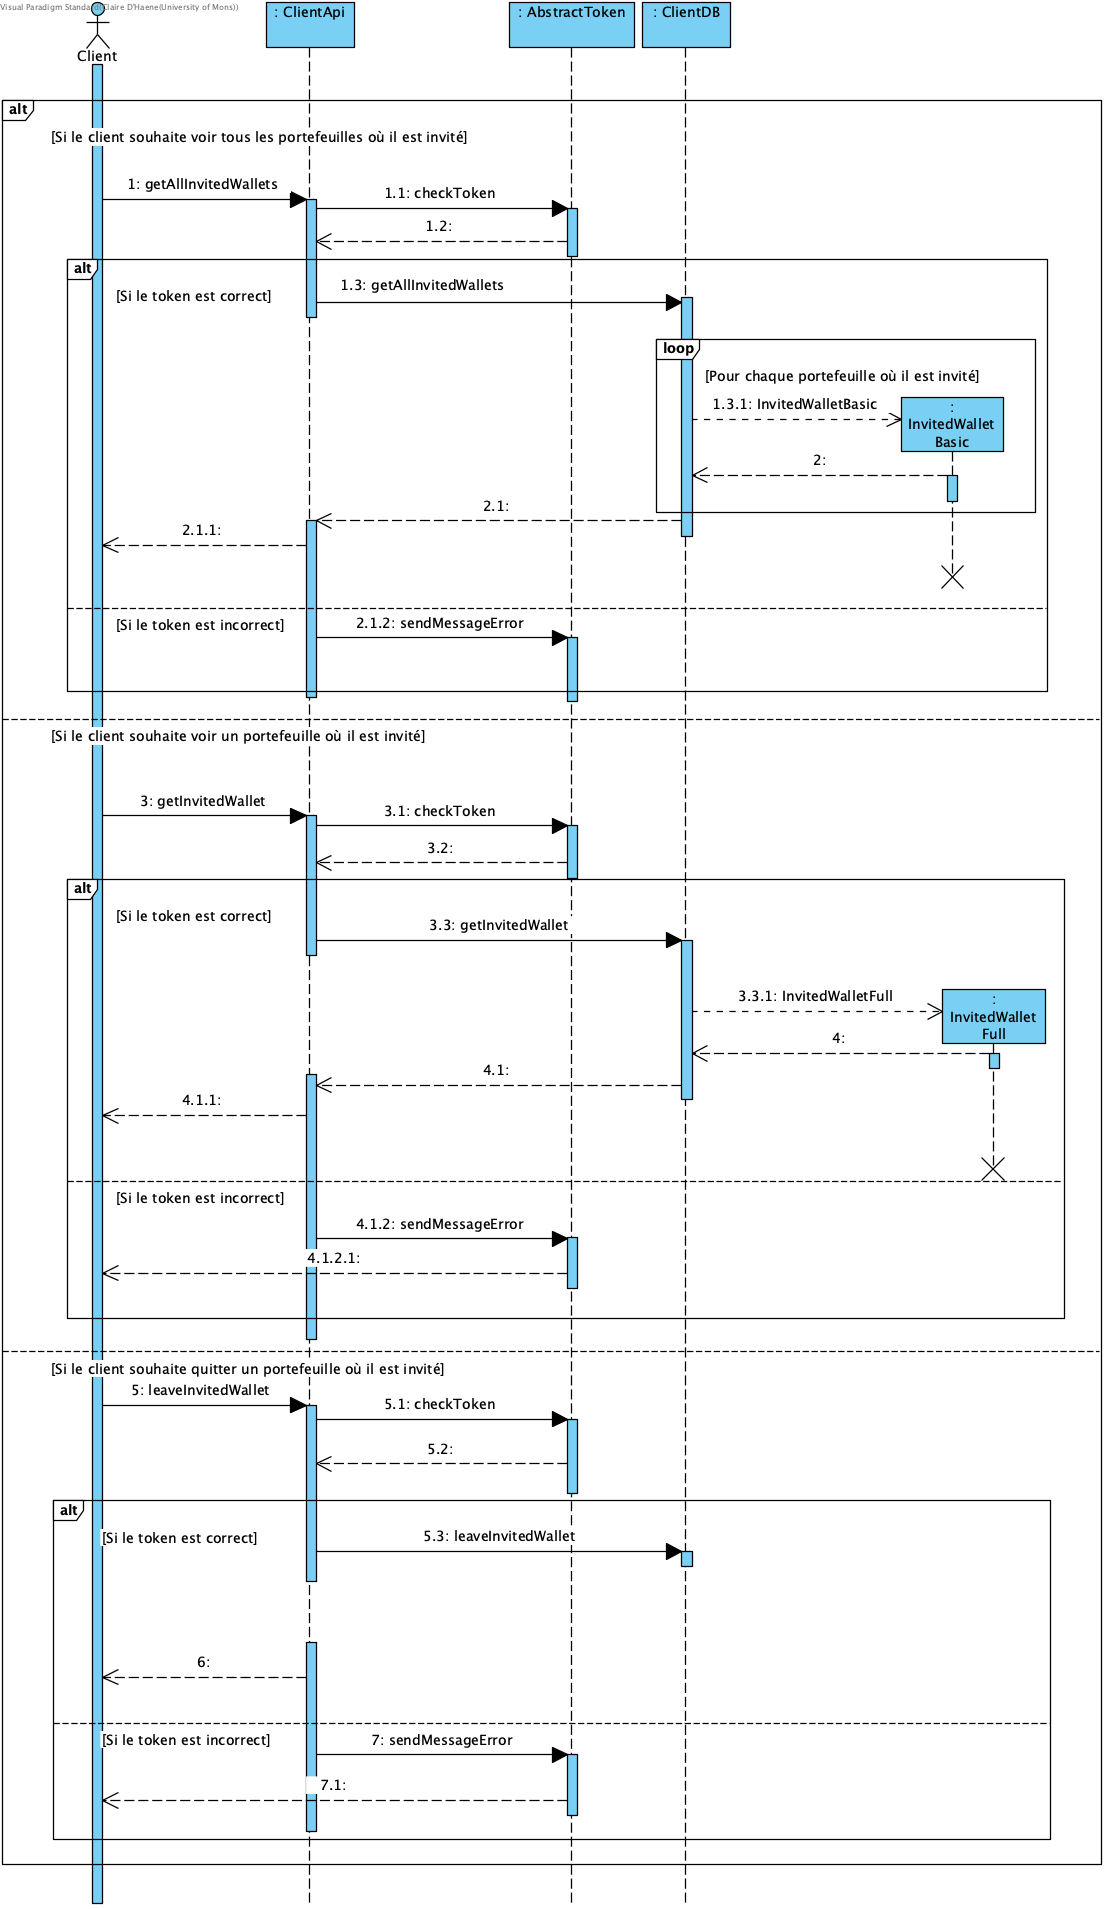
\includegraphics[height = 1.2\textwidth]{Extension-claire/Sequence-claire/img/seqOuInvité.png}
\end{figure}

\newpage

\subsubsection{Gestion des utilisateurs invités}
\begin{flushleft}
Le deuxième ajout est en partant de l'Use case \textbf{"Voir les utilisateurs invités"}. Ce dernier fonctionne de la même manière qu'expliqué précédemment pour "Voir les portefeuilles où il est invité".
\end{flushleft}
\begin{flushleft}
En effet, il y aura la méthode : 
\end{flushleft}
\begin{enumerate}
\item getAllInvitedClients si le client souhaite voir tous les utilisateurs invités. Je dois donc retourner une ArrayList de "ClientBasic".
\item mais getInvitedClient, si le client souhaite voir un utilisateur invité en particulier, ne devra pas être instanciée car toutes les informations dont un client "gestionnaire" à besoin se trouve dans un ClientBasic envoyé au préalable par la méthode getAllInvitedClients.
\end{enumerate}

\begin{flushleft}
Passons maintenant aux Use Cases \textbf{"Ajouter un utilisateur"} et \textbf{"Supprimer un utilisateur"}.
\end{flushleft}

\begin{flushleft}
Pour \textbf{ajouter un utilisateur}, j'appelle donc la méthode "addInvitedClient" de clientApi et ensuite, la méthode du même nom de ClientDB.
\end{flushleft}

\begin{flushleft}
Pour \textbf{supprimer un utilisateur}, je procède de la même manière que pour ajouter un utilisateur avec la méthode "deleteInvitedClient".
\end{flushleft}

\begin{flushleft}
Vous pouvez remarquer que ces deux méthodes ne doivent rien retourner.
\end{flushleft}

\begin{flushleft}
Au sujet de l'Use Case \textbf{"Gérer les permissions"}, si le client souhaite voir les permissions d'un invité, je ferai appel à la méthode "getPermissions" qui me retournera les permissions et s'il souhaite changer les permissions d'un invité, j'utiliserai la méthode "changePermissions".
\end{flushleft}

\begin{flushleft}
Ces deux méthodes sont d'abord appelées depuis clientApi et ensuite, de ClientDB.
\end{flushleft}

\newpage
\begin{figure}[h]
\centering
\includegraphics[height = 1.2\textwidth]{Extension-claire/Sequence-claire/img/seqUtilisateursInvités.png}
\end{figure}